\documentclass[11pt]{article}
%\usepackage[14pt]{extsizes} % для того чтобы задать нестандартный 14-ый размер шрифта
%\usepackage[utf8]{inputenc}
\usepackage{mathtext}
\usepackage[english, russian]{babel}
\usepackage{amsmath}
\usepackage{amsfonts}
\usepackage{float}
\usepackage[margin=0.8in]{geometry}
\usepackage{multirow}
\usepackage{graphicx}
\usepackage[utf8x]{inputenc} % указать кодировку русского текста
\usepackage{fancyhdr}
\usepackage{indentfirst} % отступ в первой строке абзаца
\usepackage{wrapfig}
\usepackage{placeins}
\usepackage{wrapfig}
\usepackage{caption}
\usepackage{amssymb}
\usepackage{mathtools}
\usepackage[thinc]{esdiff}

\pagestyle{fancy}
\begin{document}
\begin{titlepage}
\begin{center}
%\vspace*{1cm}
\large{\small ФЕДЕРАЛЬНОЕ ГОСУДАРСТВЕННОЕ АВТОНОМНОЕ ОБРАЗОВАТЕЛЬНОЕ\\ УЧРЕЖДЕНИЕ ВЫСШЕГО ОБРАЗОВАНИЯ\\ МОСКОВСКИЙ ФИЗИКО-ТЕХНИЧЕСКИЙ ИНСТИТУТ\\ (НАЦИОНАЛЬНЫЙ ИССЛЕДОВАТЕЛЬСКИЙ УНИВЕРСИТЕТ)\\ ФИЗТЕХ-ШКОЛА РАДИОТЕХНИКИ И КОМПЬЮТЕРНЫХ ТЕХНОЛОГИЙ}
\vfill
\line(1,0){430}\\[1mm]
\huge{Лабораторная работа 2.2.1}\\
\huge\textbf{Исследование взаимной диффузии газов}\\
\line(1,0){430}\\[1mm]
\vfill
\begin{flushright}
\normalsize{Устюжанина Мария}\\
\normalsize{\textbf{Группа Б01-107}}\\
\end{flushright}
\end{center}
\end{titlepage}
\fancyhead[L] {Работа 2.2.1}

\par \textbf{Цель работы:} 1) регимтрация зависимости концентрации гелия в воздухе от времени с помощью датчиков теплопроводности при разных начальных давлениях; 2) определение коэффициента диффузии по результатам измерений.
\par \textbf{В работе используются:} термостат; герметический сосуд, заполненный исследуемой жидкостью; отсчетный микроскоп.

\par \textbf{Введение.}

В данной работе исследуется взаимная диффузия гелия и воздуха. Давление P и температура T в условиях опыта предполагаются неизменными.

\begin{figure}[H]
\centering
\captionsetup{justification=centering}
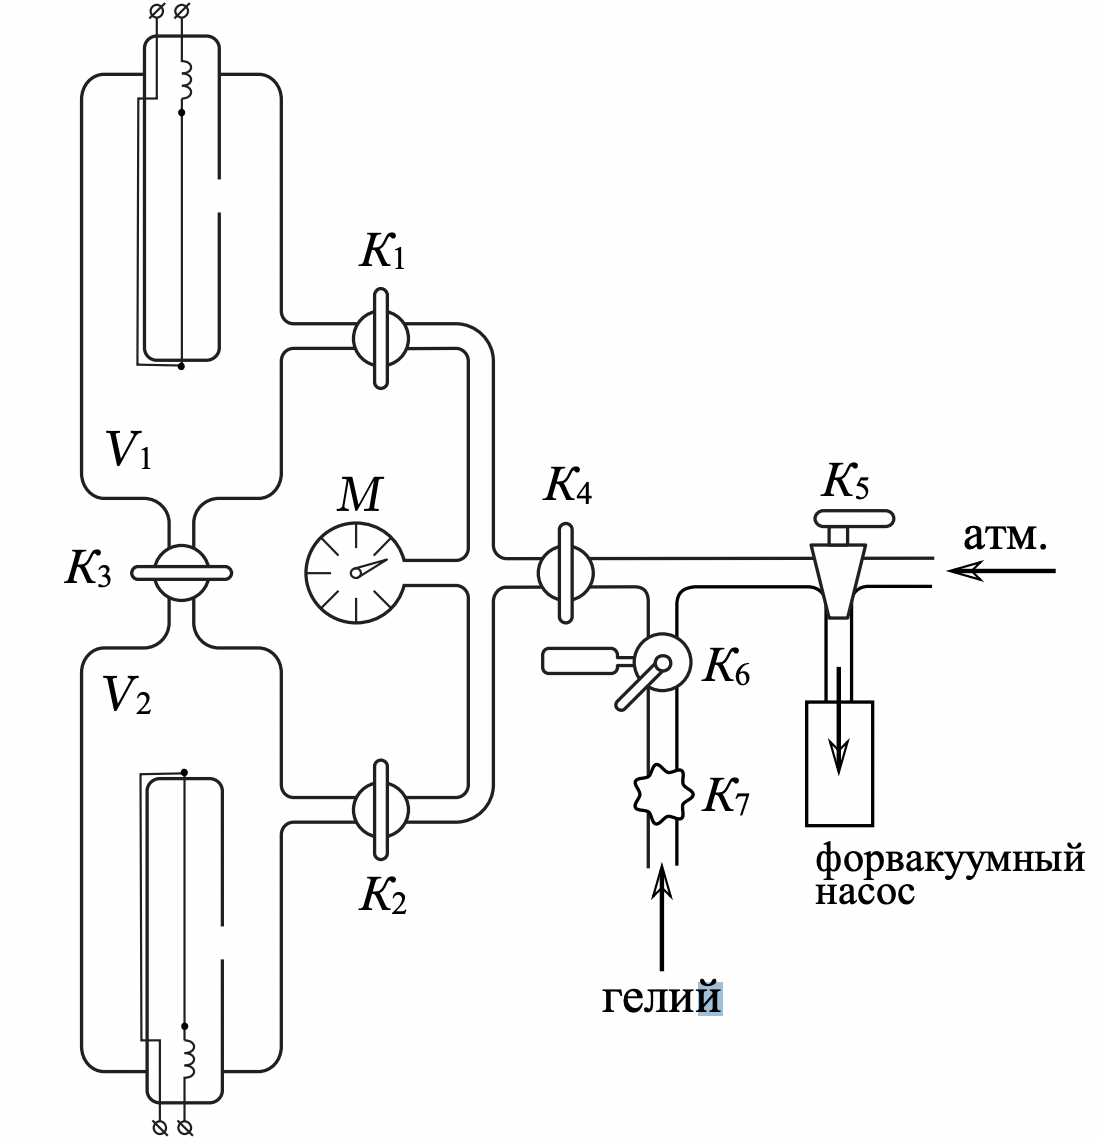
\includegraphics[width=0.5\textwidth]{pic1.png}
\caption{Схема установки}
\end{figure}

\par \textbf{Обработка данных:}

\begin{enumerate}
    \item Убедимся, что процесс диффузии подчиняется закону $\Delta n = \Delta n_0 \epsilon^{-t/\tau}$. С этой целью для каждого из рабочих давлений построим графики зависимости U(t) в логарифмическом масштабе по оси ординат. Также по угловым коэффициентам и известным геометрическим параметрам установки рассчитаем коэффициенты взаимной диффузии при выбранных рабочих давлениях. И рассчитаем погрешность.

    \medskip
     
    При $P_{раб} = 40 торр$:
    \[\frac{d(\Delta n)}{dt} = - \frac{\Delta n}{ \tau} = (2.05 \pm 0.01) \cdot 10^{-3}\frac{1}{м^3 \cdot c}\]
    \begin{figure}[H]
    \centering
    \captionsetup{justification=centering}
    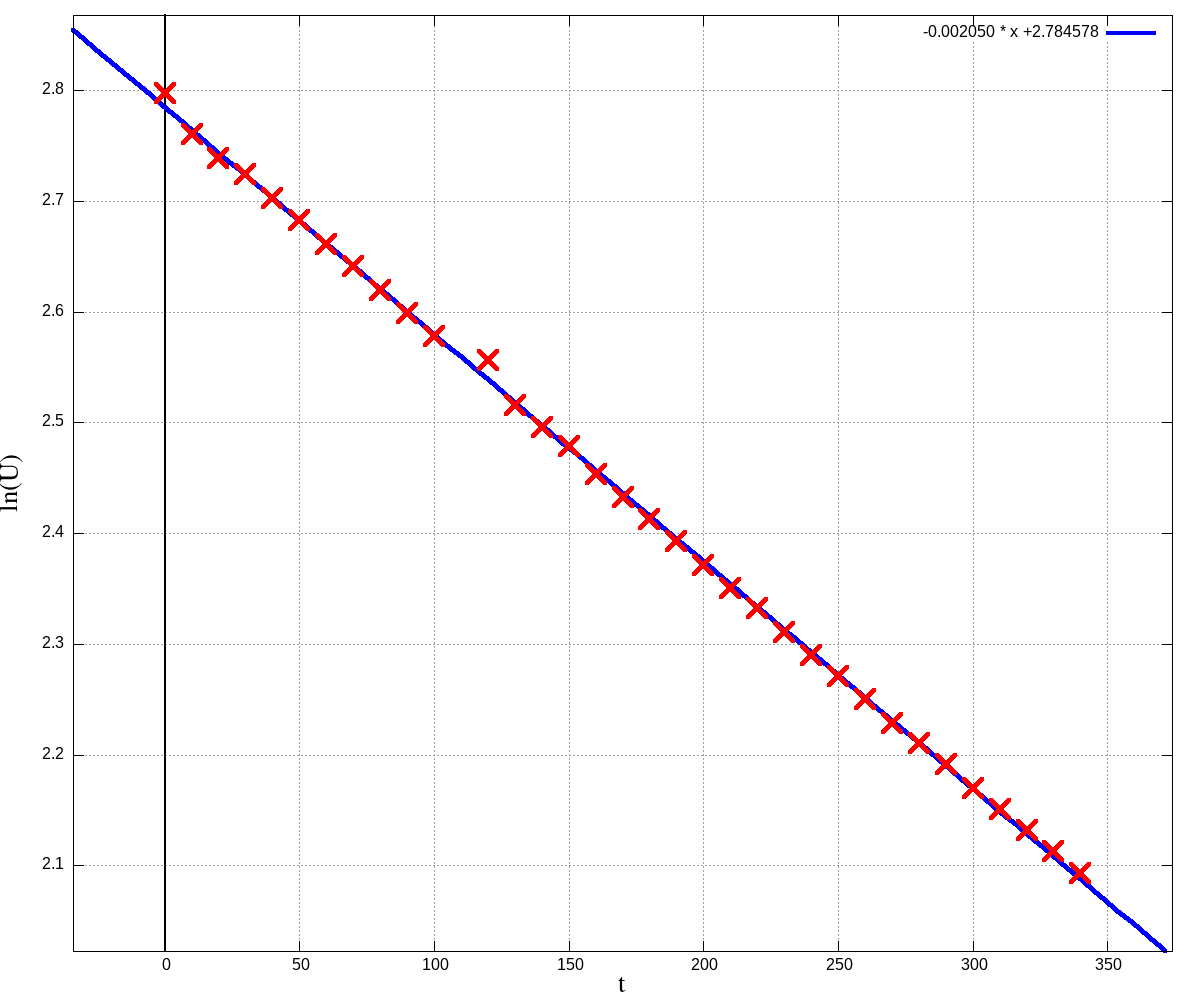
\includegraphics[width=0.5\textwidth]{1-log.res.png}
    \caption{ln(U(t)) при $P_{раб} = 40 торр$}
    \end{figure}

    \medskip
     
    При $P_{раб} = 80 торр$:
    \[\frac{d(\Delta n)}{dt} = - \frac{\Delta n}{ \tau} = (1,099 \pm 0.005) \cdot 10^{-3}\frac{1}{м^3 \cdot c}\]

    \begin{figure}[H]
    \centering
    \captionsetup{justification=centering}
    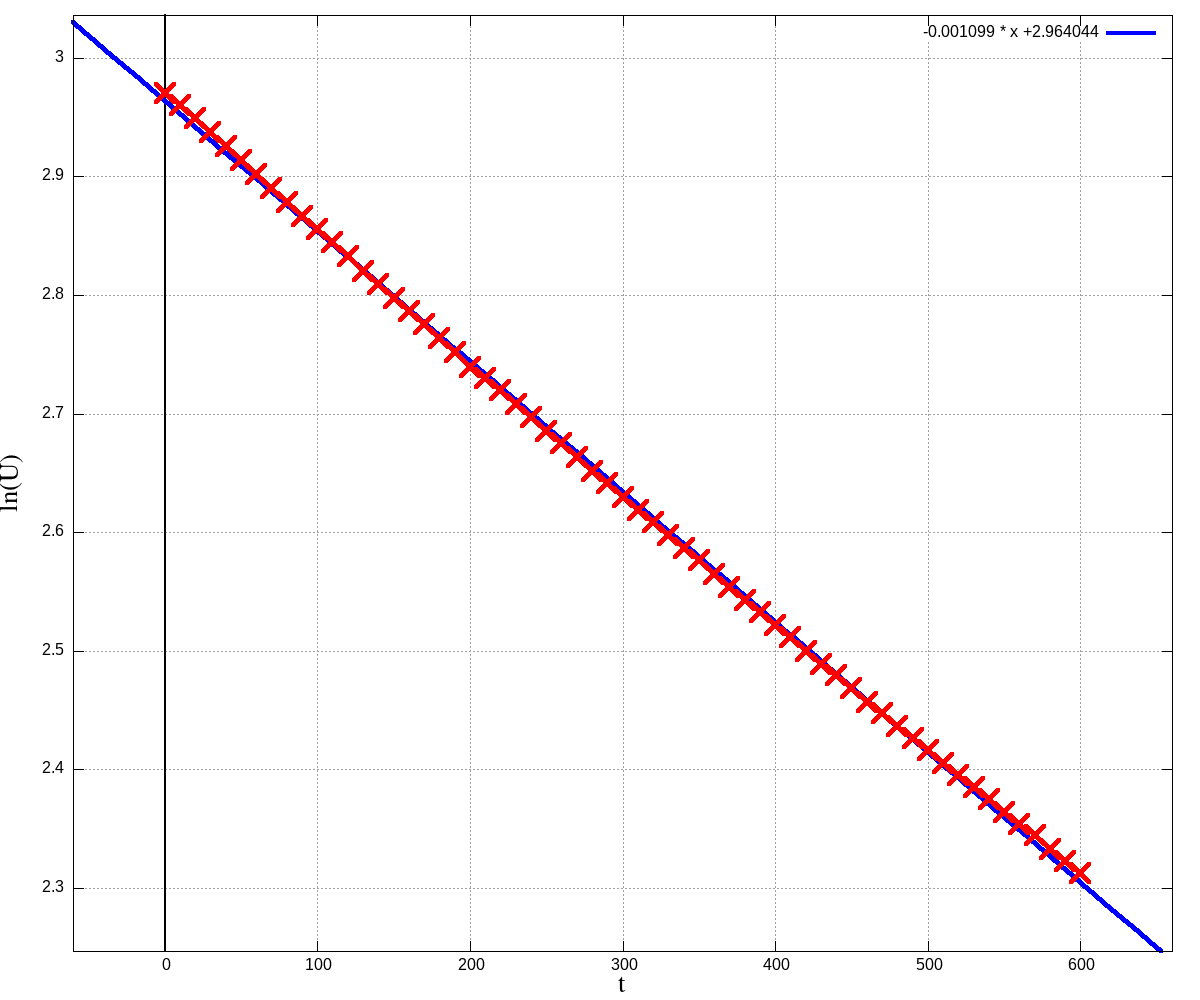
\includegraphics[width=0.5\textwidth]{2-log.res.png}
    \caption{ln(U(t)) при $P_{раб} = 80 торр$}
    \end{figure}

    \medskip
     
    При $P_{раб} = 120 торр$:
    \[\frac{d(\Delta n)}{dt} = - \frac{\Delta n}{ \tau} = (737 \pm 2) \cdot 10^{-6}\frac{1}{м^3 \cdot c}\]

    \begin{figure}[H]
    \centering
    \captionsetup{justification=centering}
    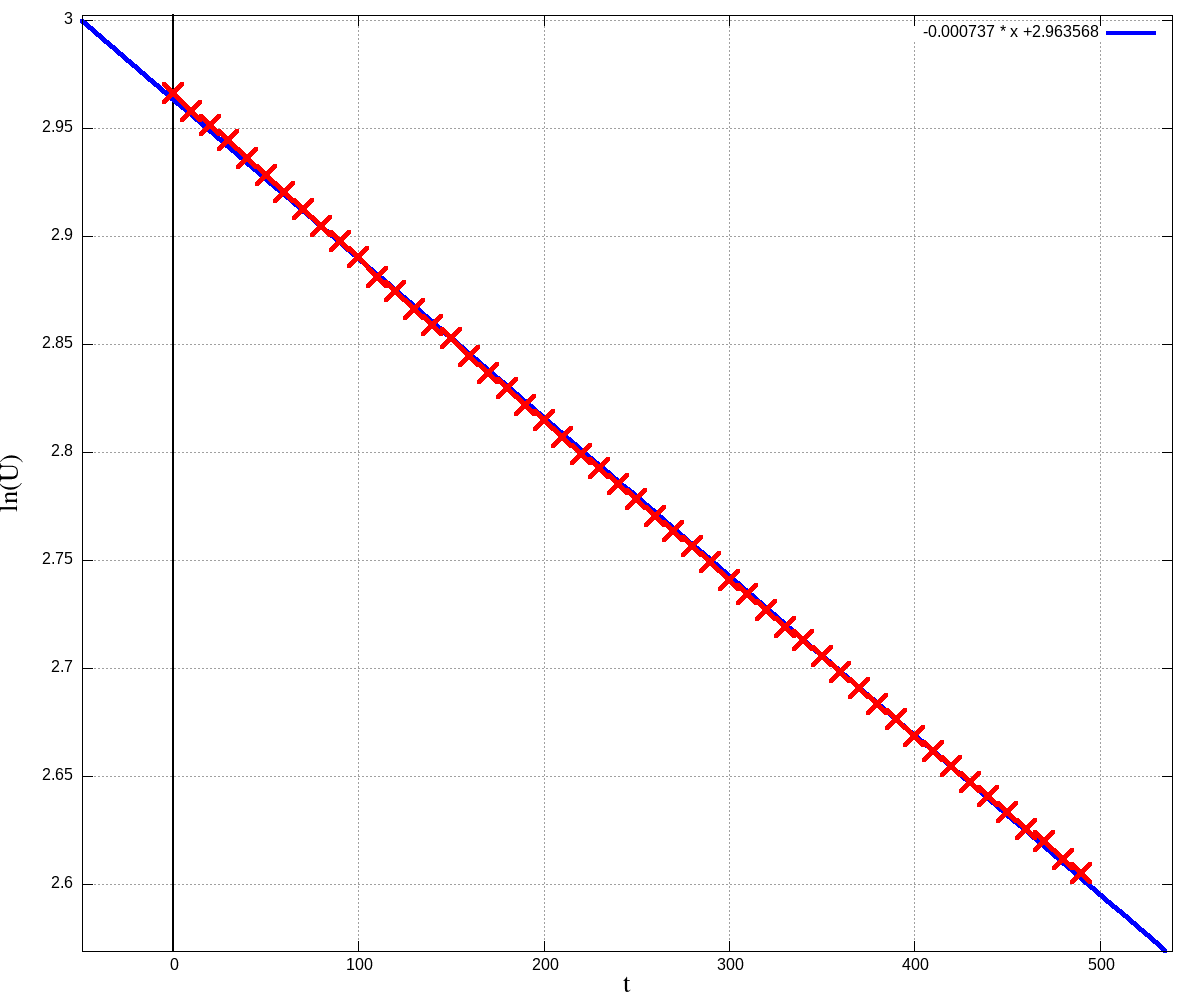
\includegraphics[width=0.5\textwidth]{3-log.res.png}
    \caption{ln(U(t)) при $P_{раб} = 120 торр$}
    \end{figure}

    \medskip
     
    При $P_{раб} = 160 торр$:
    \[\frac{d(\Delta n)}{dt} = - \frac{\Delta n}{ \tau} = ( 574\pm 2) \cdot 10^{-6}\frac{1}{м^3 \cdot c}\]

    \begin{figure}[H]
    \centering
    \captionsetup{justification=centering}
    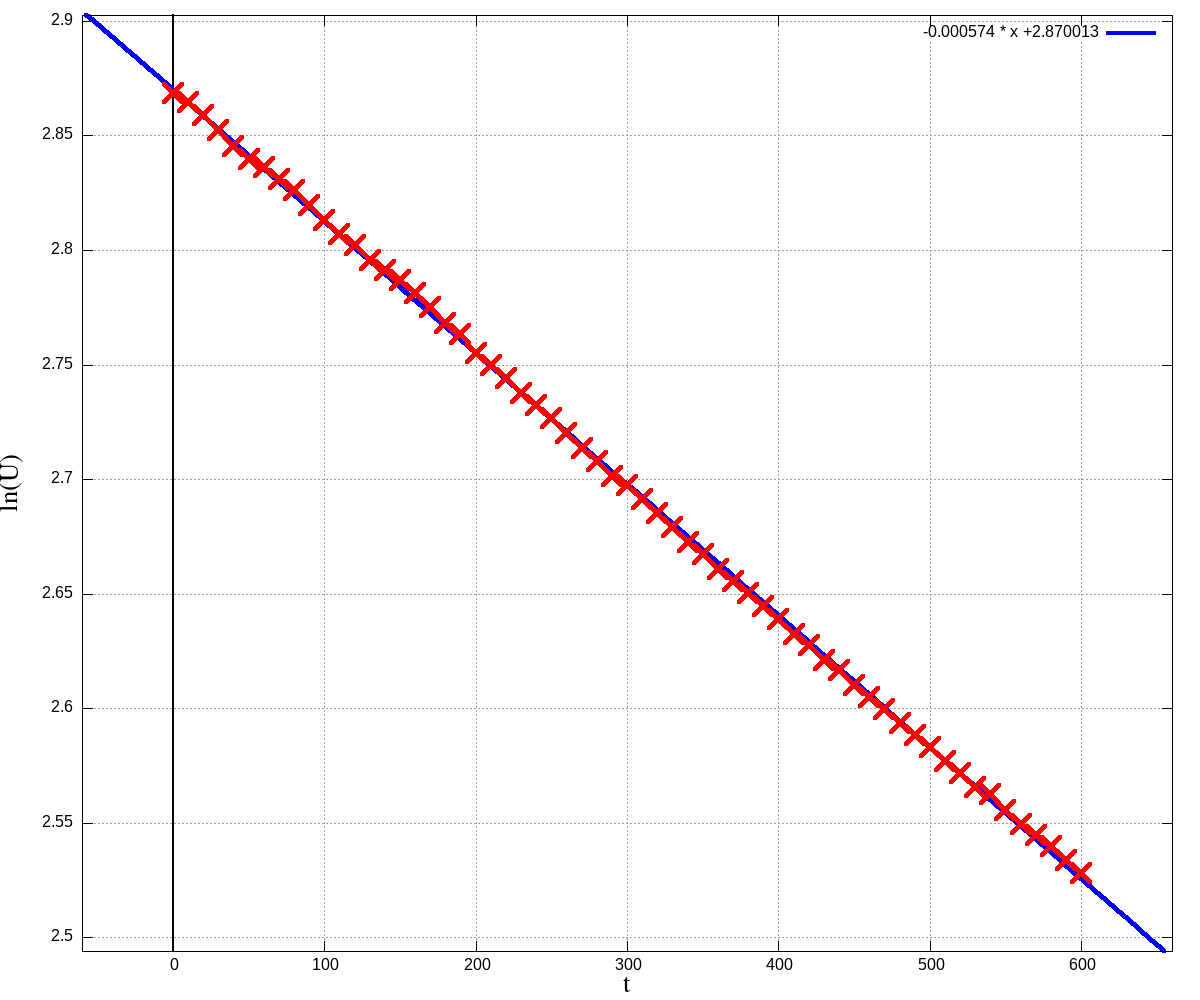
\includegraphics[width=0.5\textwidth]{4-log.res.png}
    \caption{ln(U(t)) при $P_{раб} = 160 торр$}
    \end{figure}

    \medskip

     Построим график зависимости коэффициента диффузии от обратного давления в координатах $D(\frac{1}{P})$.

    \[ D(\frac{1}{P}) = \frac{VL}{2S\tau}\]

    \medskip
    \begin{figure}[H]
    \centering
    \captionsetup{justification=centering}
    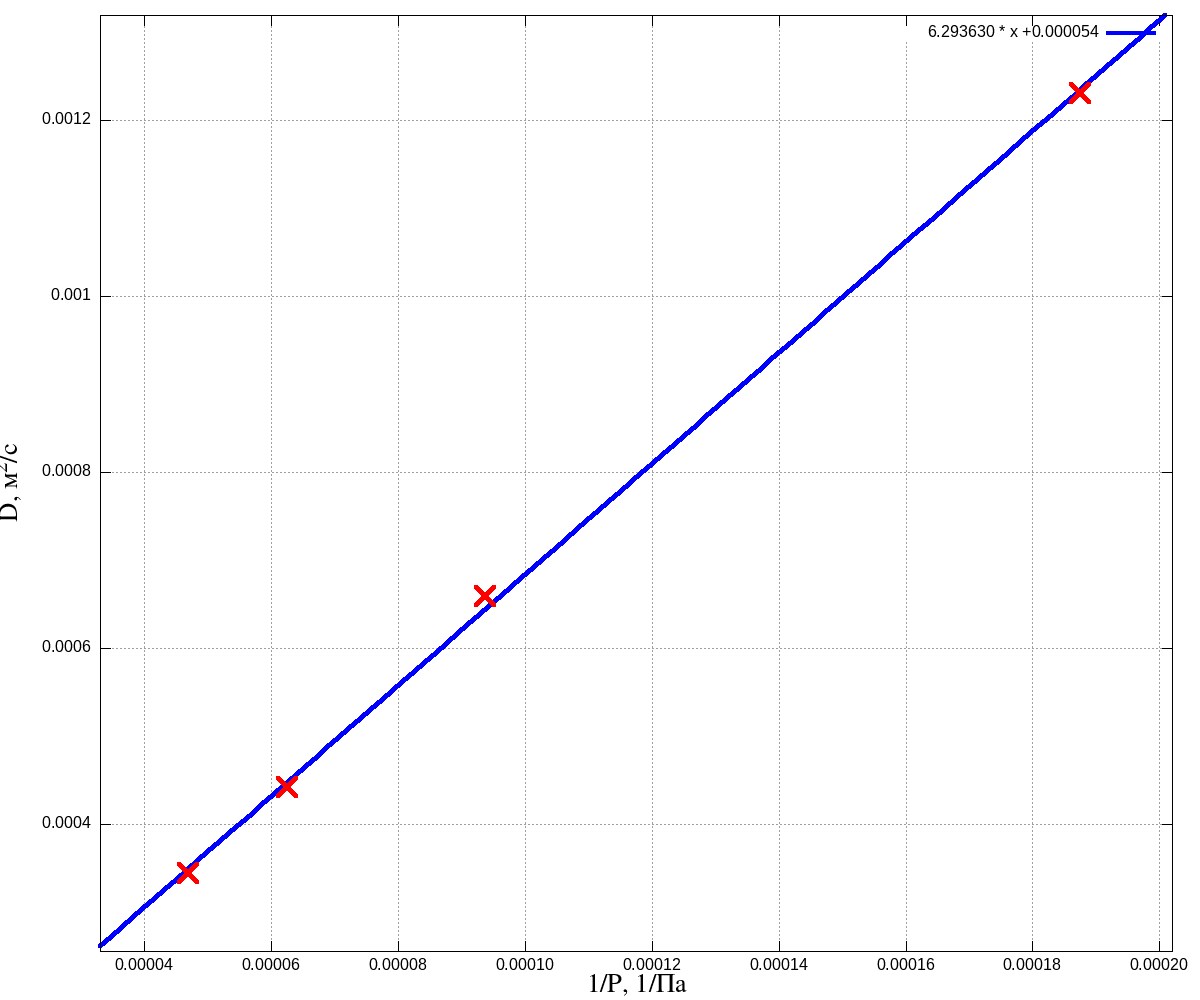
\includegraphics[width=0.5\textwidth]{graphD.png}
    \caption{$D(\frac{1}{P})$. Получилась линейная зависимость: $y = (6.29 \pm 0,07)x + 6 \cdot 10^{-5}$}
    \end{figure}


    Экстраполируем график к атмосферному давлению:
    \[D(\frac{1}{P}) = (1,23\pm 0,01)см^2/с\]




\end{enumerate}


\par \textbf{Вывод} В данной лабораторной работе была исследована зависимость коэффициента взаимной диффузии при разных рабочих давлениях. Были получены зависимости коэффициента диффузии от обратного давления в координатах $D(\frac{1}{P})$. Сравнивая полученные нами значения ($D(\frac{1}{P}) = (1,23 \pm 0,01) см^2/с$) с табличным ($D_{табл}(\frac{1}{P}) = 0,66 см^2/с$), видим, что хоть полученное значение и не совпало с табличным в пределах погрешности, оно достаточно близко к нему. 

Возможные причины расхождения теории могут заключатся в том, что температура, при которой проводился эксперимент, была около 295К, табличные значения определены для температуры 273 К, причём при более высокой температуре значения оказались выше, что и предсказывает уравнение Эйнштейна для связи коэффициента диффузии и подвижности частицы: $D = kTB$ (подвижность частицы также прямо пропорциональна значению температуры). Так что теоретически, с повышением температуры коэффициент диффузии должен повыситься, что и произошло.

\end{document}